Configurar 5 máquinas virtuales para crear el siguiente AS:

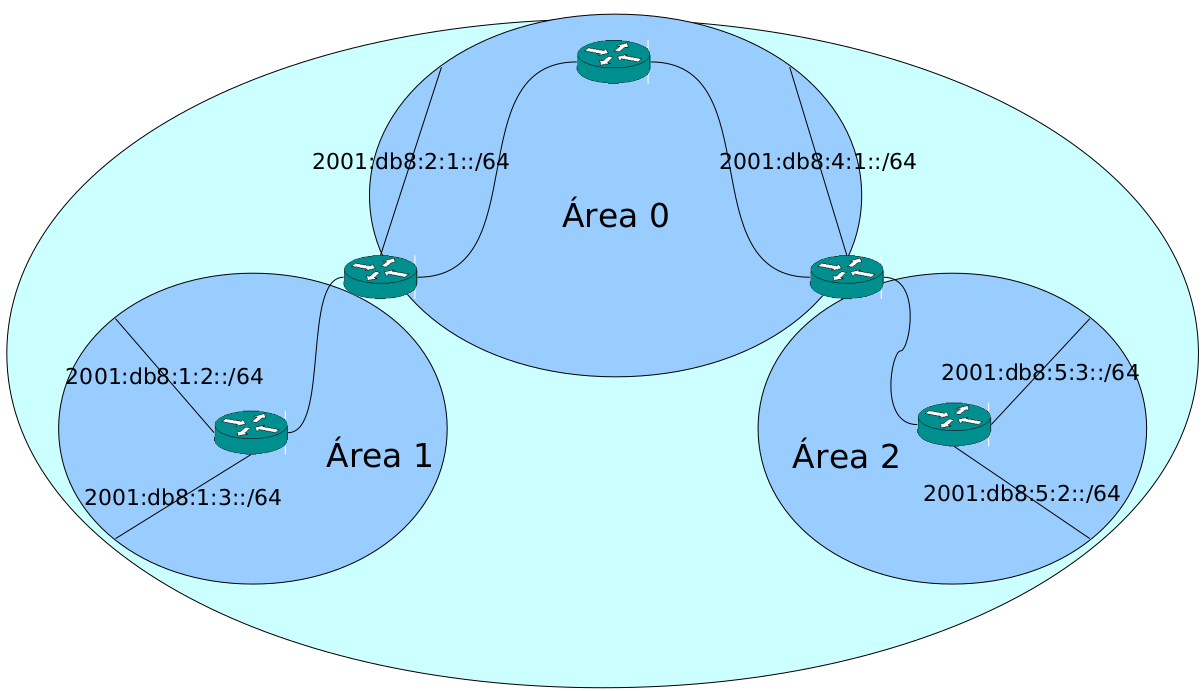
\includegraphics[width=\textwidth]{ospfv3}

\begin{minted}{bash}
 # net.conf
 defsw br12 uml1.0 uml2.0
 defsw net1 uml1.1
 defsw net2 uml1.2
 defsw br23 uml2.2 uml3.0
 defsw net3 uml2.1
 defsw br34 uml3.1 uml4.0
 defsw net4 uml4.2
 defsw br45 uml4.1 uml5.0
 defsw net5 uml5.1
 defsw net6 uml5.2
\end{minted}

\begin{minted}{bash}
  # En cuanto se inician las UML, editar el fichero /etc/quagga/daemons la línea
  ospf6d=no
  # Por
  ospf6d=yes
  # A continuación restart del servicio
  systemctl restart quagga
  # Verificar que se ospfd está corriendo
  systemctl status quagga
\end{minted}

\begin{minted}{lexer.py:IOSLexer -x}
 ! UML1 zebra.conf
 conf[igure] term[inal]
 int[erface] eth0
 no shutdown
 quit
 int[erface] eth1
 ipv6 address 2001:db8:1:3::1/64
 no shutdown
 quit
 int[erface] eth2
 ipv6 address 2001:db8:1:2::1/64
 no shutdown
 quit
 ipv6 forwarding
 exit
 write
\end{minted}

\begin{minted}{lexer.py:IOSLexer -x}
 ! UML2 zebra.conf
 conf[igure] term[inal]
 int[erface] eth0
 no shutdown
 quit
 int[erface] eth1
 ipv6 address 2001:db8:2:1::1/64
 no shutdown
 quit
 int[erface] eth2
 no shutdown
 quit
 ipv6 f[orwarding]
 exit
 write
\end{minted}

\begin{minted}{lexer.py:IOSLexer -x}
 ! UML3 zebra.conf
 conf[igure] term[inal]
 int[erface] eth0
 no shutdown
 quit
 int[erface] eth1
 no shutdown
 quit
 ipv6 f[orwarding]
 exit
 write
\end{minted}

\begin{minted}{lexer.py:IOSLexer -x}
 ! UML4 zebra.conf
 conf[igure] term[inal]
 int[erface] eth0
 no shutdown
 quit
 int[erface] eth1
 no shutdown
 quit
 int[erface] eth2
 ipv6 address 2001:db8:4:1::1/64
 no shutdown
 quit
 ipv6 f[orwarding]
 exit
 write
\end{minted}

\begin{minted}{lexer.py:IOSLexer -x}
 ! UML5 zebra.conf
 conf[igure] term[inal]
 int[erface] eth0
 no shutdown
 quit
 int[erface] eth1
 ipv6 address 2001:db8:5:3::1/64
 no shutdown
 quit
 int[erface] eth2
 ipv6 address 2001:db8:5:2::1/64
 no shutdown
 quit
 ipv6 forwarding
 exit
 write
\end{minted}

\begin{minted}{lexer.py:IOSLexer -x}
 ! UML1 ospf6d.conf
 conf[igure] term[inal]
 router ospf6
 router-id 0.0.0.1
 interface eth0 area 0.0.0.1
 interface eth1 area 0.0.0.1
 interface eth2 area 0.0.0.1
 end
 write
\end{minted}

\begin{minted}{lexer.py:IOSLexer -x}
 ! UML2 ospf6d.conf
 conf[igure] term[inal]
 router ospf6
 router-id 0.0.0.2
 interface eth0 area 0.0.0.1
 interface eth1 area 0.0.0.0
 interface eth2 area 0.0.0.0
 end
 write
\end{minted}

\begin{minted}{lexer.py:IOSLexer -x}
 ! UML3 ospf6d.conf
 conf[igure] term[inal]
 router ospf6
 router-id 0.0.0.3
 interface eth0 area 0.0.0.0
 interface eth1 area 0.0.0.0
 end
 write
\end{minted}

\begin{minted}{lexer.py:IOSLexer -x}
 ! UML4 ospf6d.conf
 conf[igure] term[inal]
 router ospf6
 router-id 0.0.0.4
 interface eth0 area 0.0.0.0
 interface eth1 area 0.0.0.2
 interface eth2 area 0.0.0.0
 end
 write
\end{minted}

\begin{minted}{lexer.py:IOSLexer -x}
 ! UML5 ospf6d.conf
 conf[igure] term[inal]
 router ospf6
 router-id 0.0.0.5
 interface eth0 area 0.0.0.2
 interface eth1 area 0.0.0.2
 interface eth2 area 0.0.0.2
\end{minted}
